\documentclass[letterpaper]{article} % DO NOT CHANGE THIS
\usepackage[submission]{aaai2027}  % DO NOT CHANGE THIS
\usepackage[hyphens]{url}  % DO NOT CHANGE THIS
\usepackage{graphicx} % DO NOT CHANGE THIS
\urlstyle{rm} % DO NOT CHANGE THIS
\def\UrlFont{\rm}  % DO NOT CHANGE THIS
\usepackage{natbib}  % DO NOT CHANGE THIS AND DO NOT ADD ANY OPTIONS TO IT
\usepackage{caption} % DO NOT CHANGE THIS AND DO NOT ADD ANY OPTIONS TO IT
\frenchspacing  % DO NOT CHANGE THIS
\usepackage{booktabs}
\usepackage{amsmath}
\usepackage{amssymb}
\usepackage{tikz}
\usetikzlibrary{arrows.meta,positioning,fit,calc}
\pdfinfo{
/TemplateVersion (2027.1)
}
\setcounter{secnumdepth}{2}

\graphicspath{{figures/}}
\newcommand{\hitat}[1]{hit@#1}
\newcommand{\mix}[1]{\texttt{#1}}

% GSR-VLM @ AAAI-27 (non-archival). 7 pages of main content; references and
% appendices unlimited. Anonymous submission mode.

\title{Decoupling What from Where:\\How Should a Small GUI Grounding Model Receive the Action Type?}
\author{Anonymous Submission}
\affiliations{}

\begin{document}

\maketitle

%% ABSTRACT: written after the Phase 9 results land.

\section{Introduction}
\label{sec:intro}

%% INTRODUCTION: framing paragraph written after the Phase 9 results land.

\section{Related Work}
\label{sec:related}

\paragraph{GUI grounding and agent models.}
Mind2Web~\citep{mind2web} and Android in the Wild~\citep{aitw} supply our episodes; AndroidControl~\citep{androidcontrol} and AndroidWorld~\citep{androidworld} extend them. SeeClick~\citep{seeclick} introduced ScreenSpot (extended by ScreenSpot-Pro~\citep{screenspotpro}), and UGround~\citep{uground} and OS-Atlas~\citep{osatlas} scale grounding pretraining. Aguvis~\citep{aguvis}, UI-TARS~\citep{uitars}, CogAgent~\citep{cogagent}, ScreenAI~\citep{screenai}, and Ferret-UI~\citep{ferretui} emit action and location together, the design our flat baseline follows; TinyClick~\citep{tinyclick} and Ferret-UI Lite~\citep{ferretuilite} work at our scale. GUI-Actor~\citep{guiactor} replaces coordinate text with an attention head, MolmoPoint~\citep{molmopoint} and GUI-AIMA~\citep{guiaima} add grounding or anchor tokens, UI-R1~\citep{uir1} rewards type and argument separately, and OmniParser~\citep{omniparser} and Set-of-Mark~\citep{som} externalize grounding.

\paragraph{Positions and spatial grounding in VLMs.}
Qwen2-VL~\citep{qwen2vl} assigns three-dimensional rotary positions (extending RoPE~\citep{roformer}) to visual tokens, computed from \texttt{input\_ids}. \citet{imrope} argue that the implicit mapping from rotary position to screen coordinate limits grounding and add explicit coordinate markers with an interleaved M-RoPE; \citet{prefill} report that a VLM's grounding decision is largely fixed during prefill. Kosmos-2~\citep{kosmos2}, Shikra~\citep{shikra}, and Ferret~\citep{ferret} teach VLMs to refer to regions. Section~\ref{sec:mrope} documents a cruder way the positions go wrong: conditioning injected through \texttt{inputs\_embeds} silently collapses the image tokens' two-dimensional layout.

\paragraph{Type-first agents.}
CoCo-Agent~\citep{cocoagent} predicts the type and then the target conditioned on it in one stream, our hard-routing variant. LiMAC~\citep{limac} places a small action transformer ahead of a LoRA-tuned Qwen2-VL-2B; the action transformer predicts the type and selects click targets over UI-element embeddings, and the VLM generates only text arguments. AutoGLM~\citep{autoglm} and Hi-Agent~\citep{hiagent} separate planning from low-level action, as do SeeAct~\citep{seeact}, Ponder\,\&\,Press~\citep{ponderpress}, and Aria-UI~\citep{ariaui}. None holds data, compute, and decoding fixed across ways of delivering the type, or intervenes on the trained model to ask whether the signal is used. Our auxiliary loss is multi-task learning in the sense of \citet{caruana}.

\section{Method}
\label{sec:method}

\begin{figure*}[t]
  \centering
  \resizebox{0.86\textwidth}{!}{% Architecture figure: two-stage factorization + the six Stage-2 conditioning
% mechanisms. \input from main.tex inside a figure environment.
% Requires: \usepackage{tikz} with libraries arrows.meta, positioning, fit, calc.
% Natural width is about 13.5 cm so that \resizebox{\linewidth} scales it by ~1.
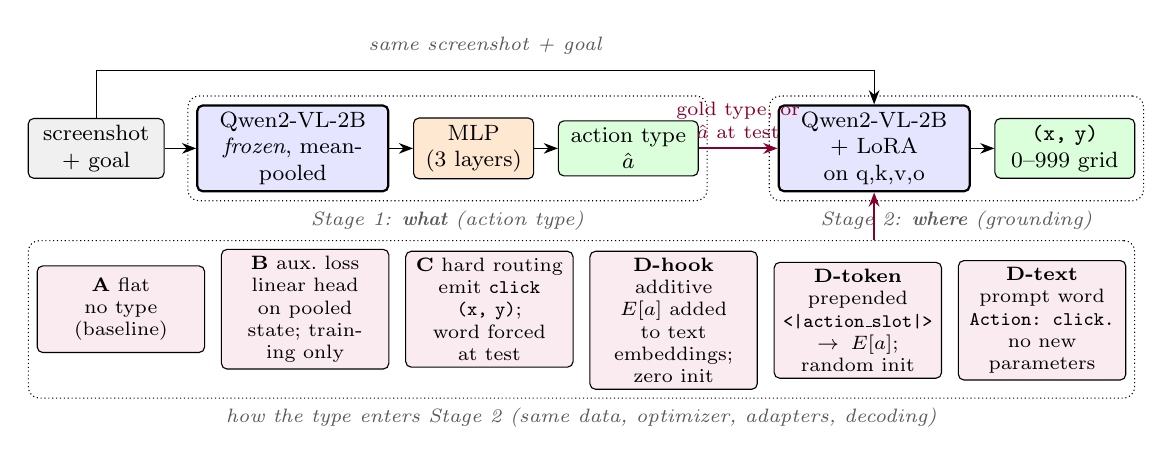
\begin{tikzpicture}[
  font=\footnotesize,
  >={Stealth[length=1.8mm]},
  box/.style={draw, rounded corners=2pt, align=center, inner sep=2.5pt, minimum height=7mm},
  inp/.style={box, fill=gray!12, text width=1.55cm},
  model/.style={box, fill=blue!10, thick, text width=2.25cm},
  head/.style={box, fill=orange!18, text width=1.35cm},
  outp/.style={box, fill=green!14, text width=1.6cm},
  mech/.style={box, fill=purple!8, text width=1.95cm, minimum height=11mm, font=\scriptsize},
  lbl/.style={font=\scriptsize\itshape, text=black!65},
  cond/.style={->, thick, purple!70!black},
  node distance=3mm,
]
  % ---------------- pipeline row ----------------
  \node[inp] (shot) {screenshot\\ + goal};
  \node[model, right=4mm of shot] (vlm1) {Qwen2-VL-2B\\ \textit{frozen}, mean-pooled};
  \node[head, right=of vlm1] (mlp) {MLP\\ (3 layers)};
  \node[outp, right=of mlp] (atype) {action type\\ $\hat a$};
  \node[model, right=10mm of atype] (vlm2) {Qwen2-VL-2B\\ + LoRA on q,k,v,o};
  \node[outp, right=of vlm2] (coord) {\texttt{(x, y)}\\ 0--999 grid};
  \node[draw, densely dotted, rounded corners, inner sep=3pt, fit=(vlm1)(mlp)(atype),
        label={[lbl]below:{Stage 1: \textbf{what} (action type)}}] (s1) {};
  \node[draw, densely dotted, rounded corners, inner sep=3pt, fit=(vlm2)(coord),
        label={[lbl]below:{Stage 2: \textbf{where} (grounding)}}] (s2) {};
  \draw[->] (shot) -- (vlm1);
  \draw[->] (vlm1) -- (mlp);
  \draw[->] (mlp) -- (atype);
  \draw[->] (vlm2) -- (coord);
  \draw[cond] (atype) -- node[above, font=\scriptsize, text=purple!70!black, align=center]
    {gold type, or\\ $\hat a$ at test} (vlm2);
  % the same inputs feed Stage 2, routed over the top
  \draw[->] (shot.north) -- ++(0,6mm) -| (vlm2.north);
  \node[lbl, anchor=south] at ($(shot.north)!0.5!(vlm2.north) + (0,6mm)$) {same screenshot + goal};

  % ---------------- mechanism row ----------------
  \coordinate (mid) at ($(shot.west)!0.5!(coord.east)$);
  \node[mech, anchor=north east] (C) at ($(mid) + (-1mm,-13mm)$)
    {\textbf{C} hard routing\\ emit \texttt{click (x, y)};\\ word forced at test};
  \node[mech, anchor=north west] (Dh) at ($(mid) + (1mm,-13mm)$)
    {\textbf{D-hook} additive\\ $E[a]$ added to text\\ embeddings; zero init};
  \node[mech, left=2mm of C] (B)
    {\textbf{B} aux.\ loss\\ linear head on pooled\\ state; training only};
  \node[mech, left=2mm of B] (A)
    {\textbf{A} flat\\ no type\\ (baseline)};
  \node[mech, right=2mm of Dh] (Dt)
    {\textbf{D-token} prepended\\ \resizebox{1.9cm}{!}{\texttt{<|action\_slot|>}}\\ $\to E[a]$; random init};
  \node[mech, right=2mm of Dt] (Dx)
    {\textbf{D-text} prompt word\\ \texttt{Action: click.}\\ no new parameters};
  \node[draw, densely dotted, rounded corners, inner sep=3pt, fit=(A)(B)(C)(Dh)(Dt)(Dx),
        label={[lbl]below:{how the type enters Stage 2 (same data, optimizer, adapters, decoding)}}] (fitbox) {};
  \draw[cond] (fitbox.north -| vlm2.south) -- (vlm2.south);
\end{tikzpicture}
}
  \caption{Two-stage pipeline. Stage~1 classifies the action type from mean-pooled frozen features. Stage~2 grounds the action to a coordinate string, and the type enters it through one of the mechanisms in the bottom row, all of which share data, optimizer, adapters, and decoding.}
  \label{fig:arch}
\end{figure*}

\subsection{Action taxonomy and grounding target}
AITW stores gestures as touch and lift points; we split them into taps (\emph{click}) and swipes (\emph{scroll}) by the normalized distance between the two, with threshold 0.04. The grounding target is the touch point normalized to $[0,1]^2$ and serialized as \texttt{(x, y)} with integers on a $0$--$999$ grid, so every target has the same token length. AITW records non-touch actions such as typing with the touch point $(-1,-1)$, and our serializer clamps it to \texttt{(0, 0)}: every \emph{type} event in a mixed training stream therefore carries the same target at the screen origin, a class the flat model must fit without being told which steps belong to it. No deployed action format creates this situation, since native formats either emit no coordinate for a type action or emit the type first. A type event's raw target is off-screen, so no model can hit it; we report every metric on click and scroll steps and repeat it over all steps in the appendix.

\subsection{Stage 1: which action}
Stage~1 runs the frozen Qwen2-VL-2B-Instruct backbone over the screenshot and the flat Stage-2 prompt, mean-pools the final hidden states over unmasked tokens into a 1536-dimensional vector, and fits a two-layer head ($1536 \to 256 \to 8$, dropout 0.1) with class-weighted cross-entropy, full-batch, for 200 epochs with no checkpoint selection, on the Stage-2 training slice. One head is fit per seed.

\subsection{Stage 2: where}
Stage~2 fine-tunes the same backbone with LoRA (rank 16, $\alpha=32$, dropout 0.05) on the query, key, value, and output projections, 4.4M trainable parameters out of 2.2B. The prompt is the screenshot, \texttt{Goal: \{goal\}}, and an instruction to predict the action coordinate; the answer is the coordinate string. With $s$ the screenshot, $g$ the goal, $a$ the action type, and $y_{1:T}$ the coordinate tokens, every variant minimizes $\mathcal{L}_{\mathrm{coord}} = -\sum_{t} \log p_\theta(y_t \mid y_{<t}, s, g, c)$ over the answer tokens, with $c$ the variant's conditioning:

\textbf{A, flat.} $c=\varnothing$: the joint-decoding design of native agent models, reduced to the grounding sub-problem.

\textbf{B, auxiliary loss.} A linear head on the mean-pooled last hidden state predicts the type during training, $\mathcal{L}_{\mathrm{B}} = \mathcal{L}_{\mathrm{coord}} + \mathrm{CE}(h_\phi(\bar z), a)$. The mean runs over the whole teacher-forced sequence, answer included, so the head can read the type off the answer (a type event's answer is \texttt{(0, 0)}). \textbf{B$'$} pools over the prompt positions only, which removes that shortcut. Nothing about the type is provided at inference to either.

\textbf{C, hard routing.} The model emits the action word before the coordinate, \texttt{click (x, y)}, as in CoCo-Agent; at test time the word is forced as a decoding prefix.

\textbf{D-hook, additive embedding.} A learned table $E \in \mathbb{R}^{8\times d}$ holds one vector per class, and a forward hook adds $E[a]$ to the embedding of every text position. $E$ starts at zero, so D-hook begins as an exact copy of A.

\textbf{D-token, prepended token.} A new token \texttt{<|action\_slot|>} sits at the start of the prompt, so it occupies a real position in \texttt{input\_ids}, and a hook replaces its embedding with $E[a]$, initialized from $\mathcal{N}(0, 0.02^2)$.

\textbf{D-text, type as a word.} The prompt begins with \texttt{Action: click.}, using pretrained word embeddings and no new parameters.

All variants share the data order, the optimizer (AdamW, learning rate $2\times10^{-5}$, weight decay 0.01, batch size 1, gradient clipping at 1.0, two epochs), and greedy decoding with 16 new tokens. The two learned tables start far from where training can move them at that rate (D-hook's rows from zero, D-token's from a random code of norm 0.78), so we also train each table at ten times the base rate, the only per-variant change in the study.

%% SETUP, RESULTS, MECHANISM, LIMITATIONS, CONCLUSION: written after the Phase 9 results land.

\bibliography{references}

\end{document}
